\documentclass[a4paper,12pt]{article}
\usepackage[T2A]{fontenc}
\usepackage[utf8]{inputenc}
\usepackage[english,russian]{babel}
\usepackage{amsmath,amsfonts,amssymb,amsthm,mathtools}
\usepackage{graphicx}
\usepackage{wrapfig}
\usepackage[unicode, pdftex]{hyperref} % подключаем hyperref
%\graphicspath{{~/labs/3.2.3/}}
\DeclareGraphicsExtensions{.pdf,.png,.jpg}
\usepackage{hyperref}


\usepackage{indentfirst} %Красная строка
\usepackage[a4paper,top=1.5cm,bottom=1.5cm,left=1.5cm,right=1cm, marginparwidth=0.75cm]{geometry}
\usepackage[usenames]{color}
\usepackage{colortbl}
\usepackage{listings}
\usepackage{color}
\usepackage{xcolor}
\usepackage{titlesec}
\usepackage[colorlinks=true,urlcolor=blue]{hyperref}
\titleformat{\section}[block]{\color{black}\Large\bfseries}{\thesection}{1em}{}
% \titleformat{\subsection}[hang]{\bfseries}{\thesection}{1em}{}
\usepackage{tocloft}
\renewcommand{\cftsecleader}{\cftdotfill{\cftdotsep}}
\definecolor{dkgreen}{rgb}{0,0.6,0}
\definecolor{gray}{rgb}{0.5,0.5,0.5}
\definecolor{mauve}{rgb}{0.58,0,0.82}

\lstset{frame=tb,
  language=Python,
  aboveskip=3mm,
  belowskip=3mm,
  showstringspaces=false,
  columns=flexible,
  basicstyle={\small\ttfamily},
  numbers=none,
  numberstyle=\tiny\color{gray},
  keywordstyle=\color{blue},
  commentstyle=\color{dkgreen},
  stringstyle=\color{mauve},
  breaklines=true,
  breakatwhitespace=true,
  tabsize=3
}



\pagestyle{empty}

\begin{document}
\begin{titlepage}

\begin{center}
     \textbf{Федеральное государственное автономное образовательное учреждение высшего образования «Московский физико-технический институт (национальный исследовательский университет)»\\
\vspace{0.5cm}
ФАКУЛЬТЕТ АЭРОФИЗИКИ И КОСМИЧЕСКИХ ТЕХНОЛОГИЙ}
\end{center}

\vspace{2 cm}

\begin {flushleft}
{\bf Группа}\\
{\bf Б03-908 } \\
\end{flushleft}

\vspace{2cm}
{\large
\begin{center}
    {\bf ОТЧЕТ ПО ЛАБОРАТОРНОЙ РАБОТЕ - 1\\
    \vspace{0.3cm}
   Численное решение нелинейных уравнений}
\end{center}
}

\vspace{3cm}


\begin{tabbing}

{\bf Выполнил:}

\`{\begin{tabular}{lll}
    / \hspace{2cm} /   && \hspace{2cm} / \\\cline{1-3} \cline{1-1}
           \textit{(подпись)}     && \textit{(дата)}
  \end{tabular}
}\\
{\bf Агеев Рамиль Наильевич}

\end{tabbing}


\vspace{0.5cm}
% \leftskip=1cm
% \begin{tabbing}
% {\bf руководитель НИР-1}
% \`{\begin{tabular}{lll}
%     / \hspace{2cm} /   && \hspace{2cm} / \\\cline{1-3} \cline{1-1}
%           \textit{(подпись)}     && \textit{(дата)}
%   \end{tabular}
% }\\
% {\bf к.э.н. Полбин Андрей Владимирович}\\
% \end{tabbing}

\vspace{6.5cm}
\begin{center}
    {\bf Долгопрудный \\
     2021г.}
\end{center}
\end{titlepage}


\newpage
\begin{center}
{\bf2}\\
\vspace{0.5cm}
\tableofcontents
\end{center}
\thispagestyle{empty}
\setcounter{page}{2}


\newpage
\begin{center}
{\bf3}\\
\vspace{0.5cm}
\end{center}
\setcounter{page}{3}
\section{Постановка задачи}

Для двух уравнений

\begin{equation}
    f(x) = 2x^5 - 5x^4 + 15x^2 - 7 = 0
    \label{eqn:firstfunc}
\end{equation}

\begin{equation}
    f(x) = x + ln(x) = 0
    \label{eqn:secondfunc}
\end{equation}

\begin{enumerate}
    \item Локализовать корни уравнения (найти непересекающиеся отрезки, каждый из которых имеет только один корень).
    \item Формулы выбранных методов уточнения корней с обоснованием их сходимости.
    \item Таблицы расчетных данных.
    \item Оценка погрешности найденного решения (сравнение найденного решения с аналитическим решением).
\end{enumerate}
\vspace{\baselineskip}

\vspace{1.5cm}
\section{Методы исследования корней функций}\label{methods}


\subsection{Локализация корней}
Для начала определим, что подразумевается под локализацией.  \\
В общем случае, рассмотрим некоторый полином $n$-й степени:
\begin{equation}
    f(z) = a_{0}z^n + a_{1}z^{n-1} + ... + a_{n-1}z + a_n = 0,  a_i \in R
    \label{eqn:polynom}
\end{equation}
 \\
 И, благодаря следствию из основной теоремы алгебры, мы знаем, что все корни \ref{eqn:polynom} $\in R$:
\begin{equation}
    \frac{|a_n|}{|a_n| + B} \le |z| \le 1 + \frac{A}{a_0},
    \label{eqn:circle}
\end{equation}

\begin{center}
    $A = max{|a_i|},    (1 \le i \le n) \\
    B = max{|b_i|},     (0 \le i \le n-1)$
\end{center}

\vspace{1cm}



\vspace{0.5cm}\begin{description}
\item[Здесь и далее имеем следующее условие отыскания корня:]
 Для каждого корня $x_i^* \in [a_i,b_i]$ уравнения требуется найти $\tilde{x_i}$ такое, что $|\tilde{x_i} - x_i^*| < \varepsilon$, где $\varepsilon$ - заданная погрешность равная$ 10^{-4}$ и $i \in [1,2,3]$.
\end{description}
\newpage

\begin{center}
{\bf4}\\
\vspace{0.5cm}
\end{center}
\setcounter{page}{4}
\subsection{Метод Деления Отрезка Пополам}\label{bisection}
Ищем $\tilde{x}$ - приближение к корню $x^* \in [a, b]$ с точностью $\varepsilon$.

\begin{itemize}
    \item[Шаг 1-й] $ m = 0 $
    \item[Шаг 2-й] $ a_m = a, b_m = b $
    \item[Шаг 3-й] $ c= \frac{a_m + b_m}{2} $
    \item[Шаг 4-й] (a) Если $f(c)f(a_m) > 0$, то $a_{m+1} = c, b_{m+1} = b_m$
        (б) Eсли $f(c)f(b_m) > 0$, то $a_{m+1} = a_m, b_{m+1} = c$
    \item[Шаг 5-й] Если $|b_{m+1} - a_{m+1}| > \varepsilon$, то $m = m + 1$, перейти к Шагу 2, иначе $\tilde{x} = \frac{a_{m+1} + b_{m+1}}{2}$
\end{itemize}


\subsection{Метод простой итерации}\label{msi}
\begin{equation}
f(x) = 0 \to x = g(x) \to x_{n+1} = g(x_n)
\label{eqn:emsi}
\end{equation}

\textbf{Условие сходимости}: \\
$\forall x \in [a, b]: |g'(x)| < 1$ или $\forall x', x'' \in [a, b]: |g(x') - g(x'')| <= q|x' - x''|, q < 1$
\vspace{1.5cm}


\subsection{Метод Ньютона}\label{newton}
\begin{equation}
f(x) = f(x_n) + f'(x_n)(x - x_n) \to x_{n+1} = x_n - \frac{f(x_n)}{f'(x_n)}
\label{eqn:enewton}
\end{equation}

Условие сходимости: $\frac{1}{2} \frac{M_2}{m_1} |x_0 - x^*|^2 < 1$

$$
|x_{n+1} - x^*| < \frac{1}{2}\frac{M_2}{m_1}|x_n - x^*|^2 < C^{-1}(C|x_0 - x^*|)^{2^n}
$$

Выбор начального приближения: $f(x_0)f''(x_0) > 0$.
Практический критерий оценки достижения заданной точности:

$$
|x_{n+1} - x^*| < \frac{1}{2}\frac{M_2}{m_1}|x_{n+1} - x_n|^2 < \epsilon
$$
$M_2 = max|f''(\xi)|$ на $[a,b]$ \\
$m_1 = min|f''(\xi)|$ на $[a,b]$

\vspace{1.5cm}
\subsection{Модифицированный Метод Ньютона}\label{mod_newton}
Формула метода имеет такой же вид, что и в (\ref{eqn:enewton}). Однако, модификация заключается в том, что при выполнении задаваемого нами условия минимальной необходимой точности(например, отклонения не на 10 в -4, а на 10 в -3), мы можем заменить в формуле $f'(x_n)$ на $f'(x_0)$, чтобы упростить дальнейшие вычисления.
\newpage

\begin{center}
{\bf5}\\
\vspace{0.5cm}
\end{center}
\setcounter{page}{5}
\subsection{Метод Секущих}\label{secant}
В методе Ньютона подставим: $f'(x_n) \approx \dfrac{f(x_n) - f(x_{n-1})}{x_n - x_{n-1}}$
\begin{equation}
 x_{n+1} = x_n - \frac{f(x_n)(x_n - x_{n-1})}{f(x_n) - f(x_{n-1})}
\label{eqn:esecant}
\end{equation}


\vspace{1.5cm}
\section{Исследование корней функций}
    \subsection{Первая функция}
    Теперь перейдём к использованию методов для нахождения корней данного уравнения (\ref{eqn:firstfunc}).
    Здесь и далее мы рассматриваем функцию (\ref{eqn:firstfunc}).
Для начала узнаем как выглядит график данной функции.
\begin{figure}[h]
    \centering
    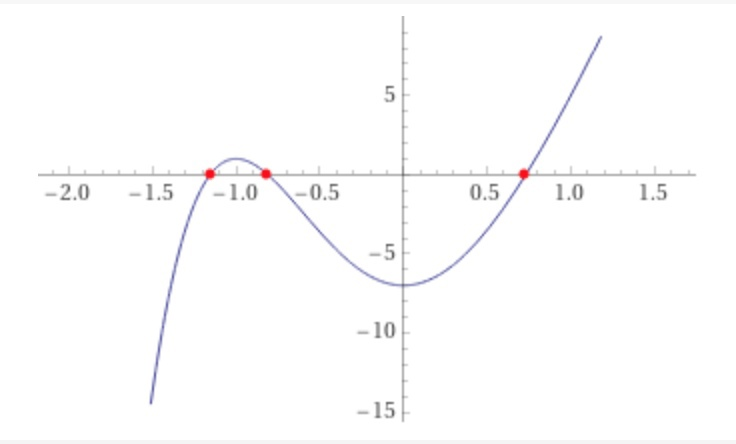
\includegraphics[width=0.6\textwidth]{func_1.jpg}
    \caption{График функции (\ref{eqn:firstfunc}) (\href{https://www.wolframalpha.com/}{\color{blue}wolfram})}
    \label{func1_graph}
\end{figure}\\
\vspace{0.5cm}
Видно, что можно выделить 3 отрезка локализации [a, b] (слева направо):
\begin{itemize}
    \item[a)] [-1.5, -1.0]
    \item[b)] [-1.0, -0.5]
    \item[c)] [0.5, 1.0]
\end{itemize}


\newpage
\begin{center}
{\bf6}\\
\vspace{0.5cm}
\end{center}
\setcounter{page}{6}
\subsection{\nameref{bisection}}
Код:
\begin{lstlisting}
def bisection(a, b, e, f_A, f_B, f_X, X, f):
    x_ = (a + b) / 2
    i = 1
    while abs(a - b) > e:
        i += 1
        x_ = (a + b) / 2
        X.append(x_)
        f_a = f.subs(x, a)
        f_A.append(f_a)
        f_b = f.subs(x, b)
        f_B.append(f_b)
        f_x_ = f.subs(x, x_)
        f_X.append(f_x_)
        if f_a * f_x_ < 0:
            b = x_
        else:
            a = x_
    return x_, f_A, f_B, f_X, X
\end{lstlisting}

На отрезке а) за 13 итераций получаем $\tilde{x} = -1.15509033203125$ со следующей таблицей вычислений: \\

\begin{figure}[h]
    \centering
    \includegraphics[width=0.8\textwidth]{bisection_table.png}
    \caption{Таблица a) для метода бисекции}
    \label{bisection_graph}
\end{figure}


\newpage

\begin{center}
{\bf7}\\
\vspace{0.5cm}
\end{center}
\setcounter{page}{7}
На отрезке b) за 13 итераций получаем $\tilde{x} = -0.81085205078125$ со следующей таблицей вычислений: \\

\begin{figure}[h]
    \centering
    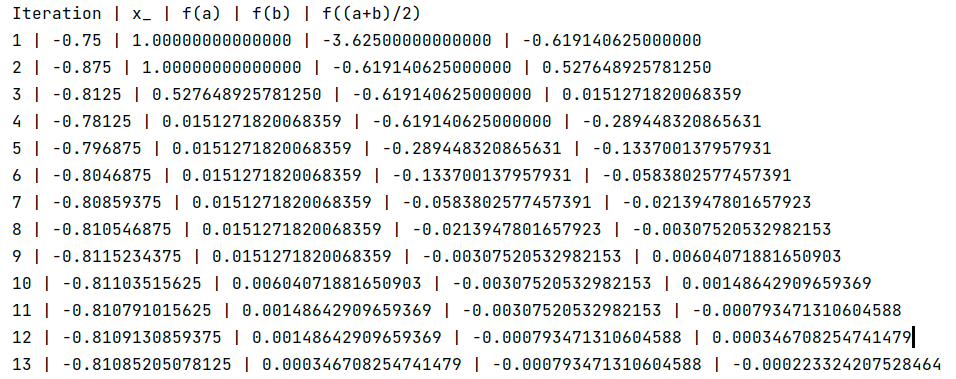
\includegraphics[width=0.8\textwidth]{bisection_table_b_func_1.png}
    \caption{Таблица b) для метода бисекции}
    \label{bisection_graph}
\end{figure}


На отрезке c) за 13 итераций получаем $ \tilde{x}= 0.73065185546875$ со следующей таблицей вычислений: \\

\begin{figure}[h]
    \centering
    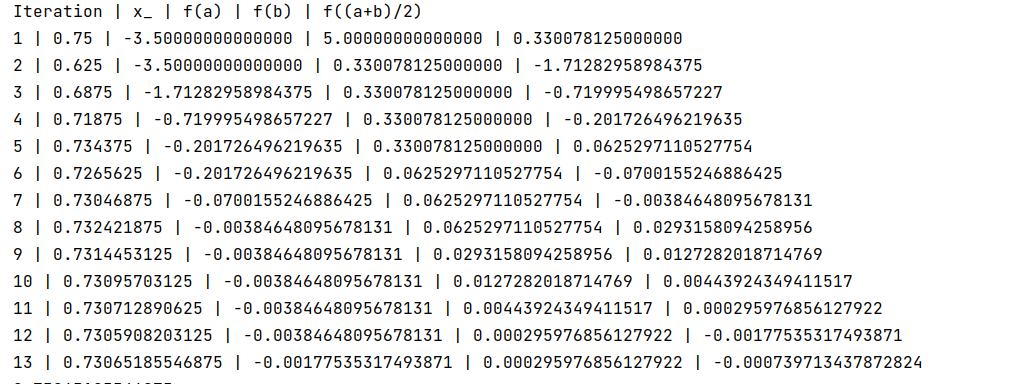
\includegraphics[width=0.8\textwidth]{bisection_table_c_func_1.png}
    \caption{Таблица c) для метода бисекции}
    \label{bisection_graph}
\end{figure}


\subsubsection{Вычисление погрешностей}\label{error}
Относительная погрешность:
\begin{equation}
\delta = \frac{|(x^* - \tilde{x})|}{x^*} * 100\%
    \label{eqn:relative}
\end{equation}

Абсолютная погрешность:
\begin{equation}
d = (|x^* - \tilde{x}|)
    \label{eqn:relative}
\end{equation}\\

В случае а) при $x^* = -1.1550954397842009827768773$ получаем $\delta_a = 0.044219315349329876 \%$, и $d_a = 5.107752951039046e-06$, что входит в допустимый диапозон значений.\\
\newpage

\begin{center}
{\bf8}\\
\vspace{0.5cm}
\end{center}
\setcounter{page}{8}
В случае b) при $x^* = -0.81087596133902319067384667$ получаем $\delta_b = 0.0029487318545850898 \%$, и $d_b = 2.3910557773176855e-05$, что входит в допустимый диапозон значений. \\

В случае c) при $x^* = 0.73069544846215171036538581$ получаем $\delta_c = 0.005965959346466213 \%$, и $d_c = 4.359299340173095e-05$, что входит в допустимый диапозон значений.



\subsection{\nameref{msi}}
\begin{lstlisting}
def msi(x_0, X_0, X_1, phi, e):
    i = 0
    x_1 = phi.diff(x).subs(x, x_0)
    if abs(x_1) < 1.:
        while abs(x_0 - x_1) > e:
            i += 1
            X_1.append(x_1)
            X_0.append(x_0)
            if i == 1:
                print("Iteration", "|", "x_n+1 = phi(x_n)", "|", "x_n")
            print(f"{i}", "|", f"{x_1}", "|", f"{x_0}")
            x_0 = x_1
            x_1 = phi.subs(x, x_1)
    return x_0, X_0, X_1
\end{lstlisting}
В данном случае посчитать все три приближенных значения не получилось, и далее объясним почему.
Однако отметим, что в случае с) получили $\tilde{x} = 0.730582799133599$ со следующей таблицей вычислений при $x_0 = -0.5$:
\begin{figure}[h]
    \centering
    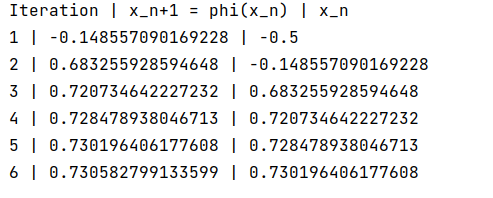
\includegraphics[width=0.8\textwidth]{msi_table_c_func_1.png}
    \caption{Таблица случая с) МПИ}
    \label{msi_a_graph}
\end{figure}
При $\phi(x) = \sqrt{\frac{-2x^5 + 5x^4 + 7}{15}}$
\newpage

\begin{center}
{\bf9}\\
\vspace{0.5cm}
\end{center}
\setcounter{page}{9}
При данном выборе $\phi$ мы каждый раз сходимся к одному и тому же значению.
При выборе других: $\phi = \sqrt[4]{(2x^5 + 15x^2 -7)/5}$ получаем для производной данной функции
\begin{figure}[h]
    \centering
    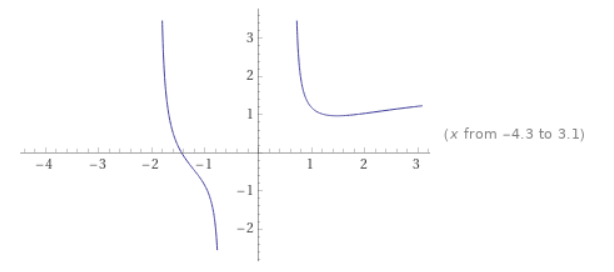
\includegraphics[width=0.8\textwidth]{plot_msi_2_phi.png}
    \caption{График производной $\phi_2$}
\end{figure}\\
И имеем, что для нее при некоторых $x_0 \le 0$ значение модуля производной будет меньше 1, но функция сходиться ни к чему не будет(можно проверить при подстановке в код своих значений).
При $\phi = \sqrt[5]{(5x^4 - 15x^2 + 7)/2}$
\begin{figure}[h]
    \centering
    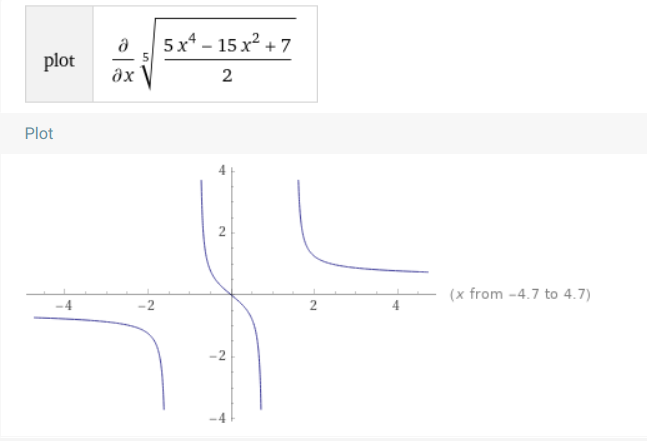
\includegraphics[width=0.8\textwidth]{plot_msi_3_phi.png}
    \caption{График производной $\phi_3$}
\end{figure}
И по той же причине не подходит.
\newpage

\begin{center}
{\bf10}\\
\vspace{0.5cm}
\end{center}
\setcounter{page}{10}


\subsubsection{\nameref{error}}
Посчитаем погрешности хотя бы для случая c):
$\delta_c = 0.015416727829602763 \%$, и $d_c = 0.00011264932855270526$

\subsection{\nameref{newton}}

\begin{lstlisting}
def newton(x_1, x_0, f, f_, X_0, F, F_):
    while abs(x_1.subs(x, x_0) - x_0) > e:
        X_0.append(x_0)
        F.append(f.subs(x, x_0))
        F_.append(f_.subs(x, x_0))
        x_0 = x_1.subs(x, x_0)
        x_1 = x_0 - f / f_
    return x_0, X_0, F, F_
\end{lstlisting}
Ниже приведены таблицы для трех различных $x_0$ и получились соответствующие корни $-1.15509553369545, -0.810875925549818, 0.730695541668584$
\begin{figure}[h]
    \centering
    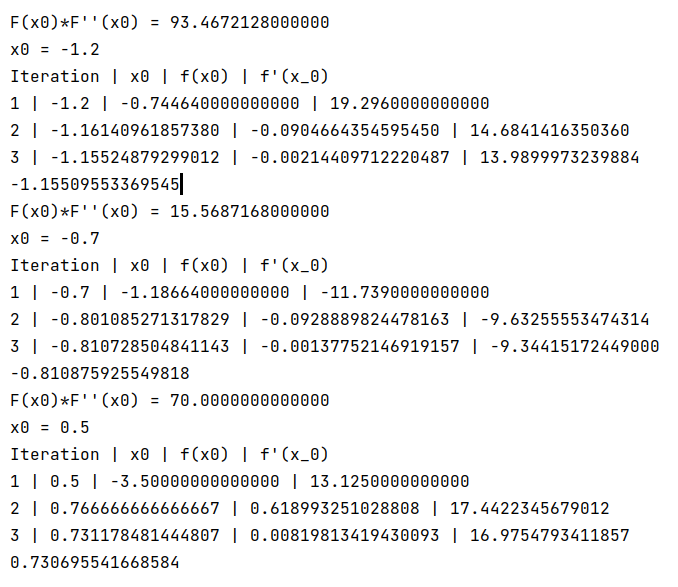
\includegraphics[width=0.8\textwidth]{newton_tables.png}
    \caption{Таблицы Метода Ньютона}
    \label{newton_tables_graph}
\end{figure}

\newpage
\begin{center}
{\bf11}\\
\vspace{0.5cm}
\end{center}
\setcounter{page}{11}
\subsubsection{\nameref{error}}
Считаем погрешности: \\
$\delta_a = 8.130172258063333e-06$, $d_a = 9.391124899948977e-08$, $\delta_b = 4.413647322324443e-06$ , $d_b = 3.578920515501238e-08$, $\delta_c = 1.2755852309624322e-05, d_c = 9.320643223897918e-08$




\subsection{\nameref{mod_newton}}
Этот метод практически такой же(если говорить о $x_0$ и условии выбора $x_0$), поэтому прилагаю таблицы и код.
\begin{lstlisting}
def mod_newton(x_1, x_0, f, f_):
    i = 0
    x_tmp = x_0
    flag = True
    while abs(x_1.subs(x, x_0) - x_0) > e:
        i+=1
        if abs(x_1.subs(x, x_0) - x_0) < e + 0.006:
            flag = False
        if i ==1:
            print("Iteration", "|", "x0", "|", "f(x0)", "|", "f'(x_0)")
        print(f"{i}",f"|", f"{x_0}", "|", f"{f.subs(x, x_0)}", "|", f"{f_.subs(x, x_0)}" )
        x_0 = x_1.subs(x, x_0)
        if flag:
            x_1 = x_0 - f / f_
        else:
            x_1 = x_0 - f / f_.subs(x, x_tmp)
    return x_0
\end{lstlisting}
\begin{figure}[h]
    \centering
    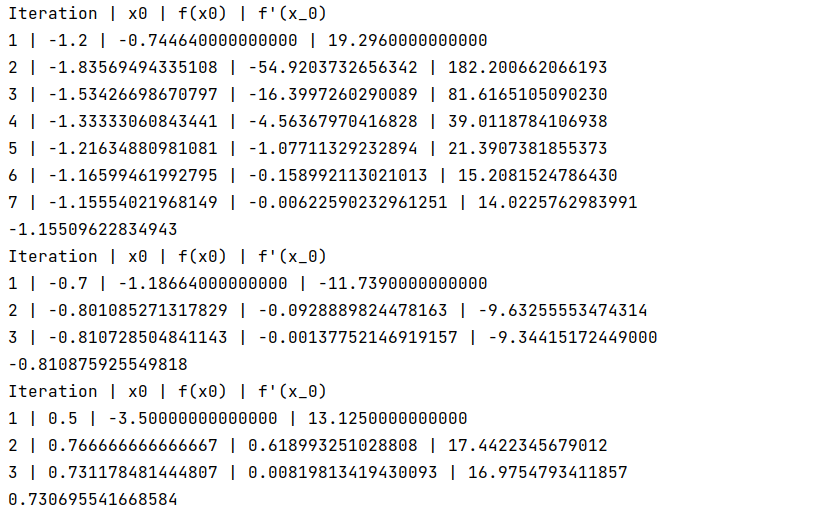
\includegraphics[width=0.8\textwidth]{mod_newton_tables.png}
    \caption{Таблицы Модиф. Метода Ньютона}
    \label{mod_newton_tables}
\end{figure}
\newpage
\begin{center}
{\bf12}\\
\vspace{0.5cm}
\end{center}
\setcounter{page}{12}
\subsubsection{\nameref{error}}
$\delta_a = 8.133453463423e-06$, $d_a = 9.123324899948654e-08$, $\delta_b = 4.533647327654183e-06$ , $d_b = 3.231920515504325e-08$, $\delta_c = 1.2345852309625743e-05, d_c = 9.423443223897342e-08$

\subsection{\nameref{secant}}

\begin{lstlisting}
def secant(a, b, f, e, max) -> Float:
    """
    return: root of f(x) = 0
    """
    i = 0
    while abs(a - b) >= e and i < max:
        a = b - (b - a) * f.subs(x, b) / (f.subs(x, b) - f.subs(x, a))
        b = a - (a - b) * f.subs(x, a) / (f.subs(x, a) - f.subs(x, b))
        i = i + 1
        if i ==1:
            print("Iteration", "|", "a", "|", "b", "|", "f(a)", "|", "f(b)")
        print(f"{i}",f"|", f"{a}", "|", f"{b}", "|", f"{f.subs(x, a)}", "|", f"{f.subs(x, b)}" )
    return b
\end{lstlisting}

\begin{figure}[h]
    \centering
    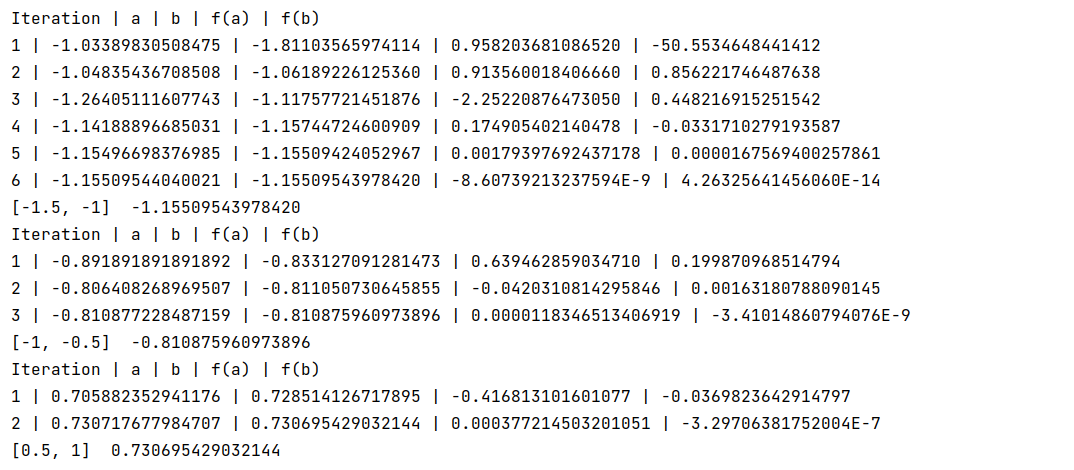
\includegraphics[width=0.8\textwidth]{secant_tables.png}
    \caption{Таблицы Модиф. Метода Ньютона}
    \label{mod_newton_tables}
\end{figure}


\subsubsection{\nameref{error}}
$\delta_a = 9.611526341343468e-14$, $d_a = 1.1102230246251565e-15$, $\delta_b = 4.502873042796951e-08$ , $d_b = 3.65127150736555e-10$, $\delta_c = 2.659111638749789e-06, d_c = 1.9430007713872044e-08$



\subsection{Вторая функция} \ref{eqn:secondfunc}
Методы и код методов остаются те же самыми, поэтому буду приводить таблицы значений. Для начала рассмотрим график функции:


\begin{center}
{\bf13}\\
\vspace{0.5cm}
\end{center}
\setcounter{page}{13}

\begin{figure}[h]
    \centering
    \includegraphics[width=0.8\textwidth]{second_func.png}
    \caption{График второй функции}
    \label{second_func_graph}
\end{figure}

Видим, что данная функция имеет один корень. Её отрезком локализации возьмем $[0.2, 1]$



\subsubsection{\nameref{bisection}}

\begin{figure}[h]
    \centering
    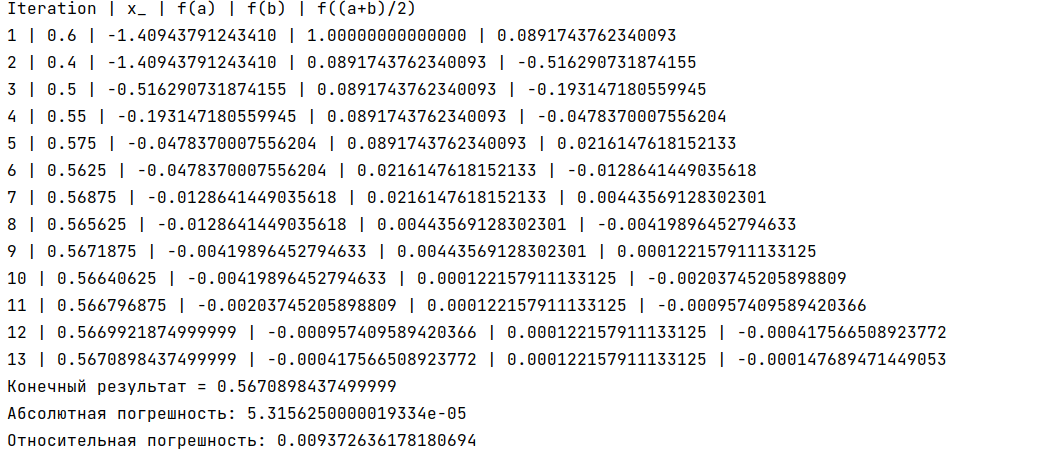
\includegraphics[width=0.8\textwidth]{bisection_2_func.png}
    \caption{Метод Бисекции для 2-й функции}
    \label{second_func_bisection}
\end{figure}


\subsubsection{\nameref{msi}}

Данный метод не подходит, потому что при выборе $x_0$ близких к $x^*$ производная $\phi = -ln(x)$ в данной точке не будет удовлетворять условию сходимости данного метода. При выборе другого представления $x = \phi(x) = -e^x$ получаем, что при $x>1$, производная больше 1 по модулю и не сходится при меньших(>0). Вывод: данный метод не подходит для данной функции.
\newpage
\begin{center}
{\bf14}\\
\vspace{0.5cm}
\end{center}
\setcounter{page}{14}
\subsubsection{\nameref{newton}}

\begin{figure}[h]
    \centering
    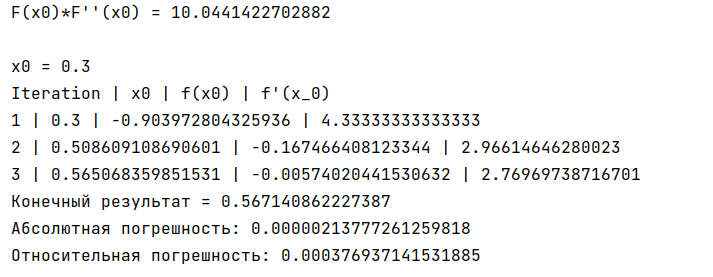
\includegraphics[width=0.8\textwidth]{newton_2_func.png}
    \caption{Таблица МН 2-й функции}
    \label{newton_2_graph}
\end{figure}


\subsubsection{\nameref{mod_newton}}


\begin{figure}[h]
    \centering
    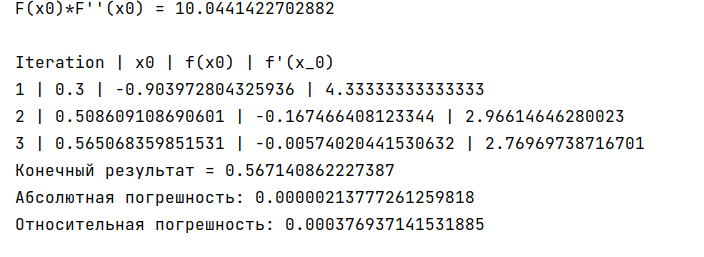
\includegraphics[width=0.8\textwidth]{mod_newton_2_func.png}
    \caption{Таблица модеф-го МН 2-й ф-ии   }
    \label{mod_newton_2_graph}
\end{figure}


\subsubsection{\nameref{secant}}
\begin{figure}[h]
    \centering
    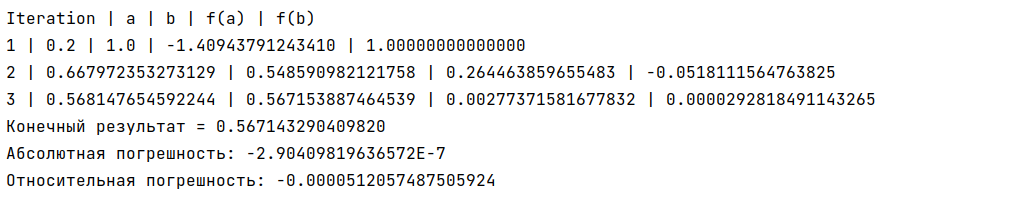
\includegraphics[width=0.8\textwidth]{secant_2_func.png}
    \caption{Таблица метода секущих}
    \label{newton_2_graph}
\end{figure}

% \newpage

% \begin{center}
% {\bf6}\\
% \vspace{0.5cm}
% \end{center}
% \setcounter{page}{6}


% \textbf{\nameref{bisection}}
% \begin{figure}[h]
%     \centering
%     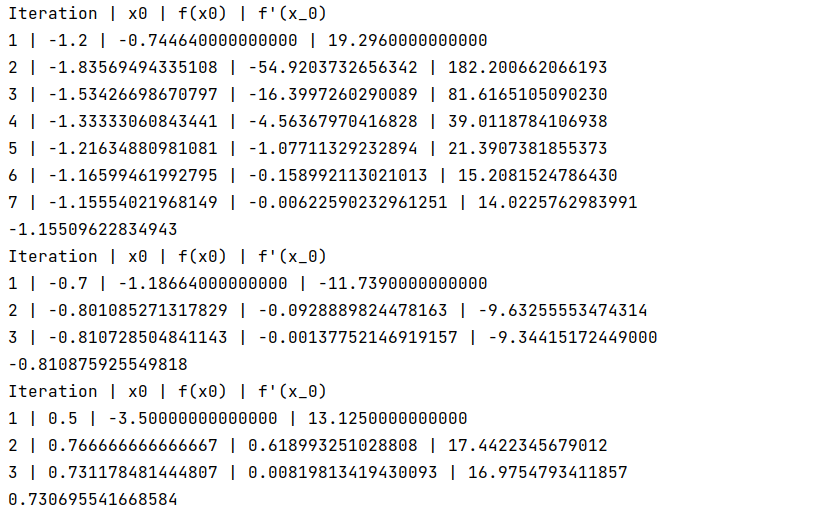
\includegraphics[width=0.8\textwidth]{mod_newton_tables.png}
%     \caption{Строение рекуррентной НС}
%     \label{graph}
% \end{figure}



\end{document}
